\begin{abstract}
	In this report we present a number of models describing neuronal dynamics.
	Firstly we present a simple leaky integrate-and-fire model, a fully deterministic representation of the neuron, which equates it to a single resistance-capacitance circuit.
	The ability of generating spikes in this model is hard coded posing a threshold on the membrane potential.
	This model is then expanded as to model supra-threshold dynamics, adding to the model a new state variable, the inter-spike time, allowing to model time-dependent changes in the systems parameter.
	The deterministic model is expanded again to model spike-rate adaptation and synaptic transmission.
	The deterministic representation of the model doesn't allow to explore channels opening and closing, so we introduce a piecewise stochastic representation for the model.
	The neuron is then modelled as an hybrid system in which the voltage evolves deterministically in between stochastic channel events.
	We implemented two representation for the stochastic model: the random time change and Gillespie's direct method.
	Finally we explored how these two representation differs and propose a methodology to fit them to experimental data.
\end{abstract}
\chapter{Introduction}


\section{Stochastic representations}

	\subsection{Random time change representation}
	Consider a model of a system with states $A$ for closed and $B$ for open of an ion channel.
	The dynamics of the system are modeled assuming that the dwell times in the two states are determined by independent exponential random variables with parameters $\alpha$ and $\beta$:

	$$A\xleftrightharpoons[\beta]{\alpha}B$$

	The probability that a closed channel opens in the next increment of time $\Delta s$ is assumed $\alpha\Delta s + o(\Delta s)$, while the probability that an open channel closes is assumed $\beta\Delta s + o(\Delta s)$.
	This model can be described mathematically by a chemical master equation, that for the two states model is:

	$$\begin{cases}\frac{d}{dt}p_{x_0}(A, t) = -\alpha p_{x_0}(A, t) + \beta p_{x_0}(B, t)\\\frac{d}{dt}p_{x_0}(B, t) = -\beta p_{x_0}(B, t) + \alpha p_{x_0}(A, t)\end{cases}$$

	Where:

	\begin{itemize}
		\item $p_{x_0}(x, t)$ is the probability of being in state $x\in \{A, B\}$ at time $t$ given the initial condition $x_0$.
		\item $x_0$ is the initial condition.
	\end{itemize}

	The chemical master equation is a linear ODE governing the dynamical behaviour of the probability distribution of the model and does not provide a stochastic representation for a particular realization of the process.
	To reconstruct  a path-wise representation let:

	\begin{itemize}
		\item $R_1(t)$ be the number of times $A\rightarrow B$ has taken place by time $t$.
		\item $R_2(t)$ be the number of times $B\rightarrow A$ has taken place by time $t$.
		\item $X_1(t)\in\{0,1\}$ be $1$ if the channel is closed at time $t$ and zero otherwise.
		\item $X_2(t)=1-X_1(t)$ be $1$ if the channel is open at time $t$ and zero otherwise.
		\item $X(t) = \begin{pmatrix}X_1(t) & X_2(t)\end{pmatrix}^T$.
	\end{itemize}

	Now:

	$$X(t) = X(0) + R_1(t)\begin{pmatrix}-1\\1\end{pmatrix} + R_2(t)\begin{pmatrix}1\\-1\end{pmatrix}$$

	The counting processes $R_1$ and $R_2$ are represented as unit-rate Poisson processes.
	A unit-rate Poisson process can be constructed considering:

	\begin{itemize}
		\item $\{e_i\}_{i=1}^{\infty}$ independent exponential random variables with a parameter of $1$.
		\item $\tau=e_1, \tau_2 = \tau_1+e_2, \dots, \tau_n = \tau_{n-1} + e_n$.
	\end{itemize}

	The associated unit-rate Poisson processes $Y(s)$ is the counting process determined by the number of points $\{\tau_i\}_{i=1}^{\infty}$ that come before $s \ge 0$.
	Let $\lambda:[0, \infty[\rightarrow\mathbb{R}_{\ge 0}$ be the rate of movement along the time axis, then the number of points observed by time $s$ is:

	$$Y\biggl(\int_0^{s}\lambda(r)dr\biggr)$$

	From the basic properties of exponential random variables, whenever $\lambda(s)>0$, the probability of seeing a jump within the next small increment of time $\Delta s$ is:

	$$P\biggl(Y\biggl(\int_{0}^{s+\Delta s}\lambda(r)dr\biggr)-Y\biggl(\int_{0}^{s}\lambda(r)dr\biggr)\ge 1\biggr)\sim \lambda(s)\Delta s$$

	Thus the propensity for seeing another jump is $\lambda(s)$.
	Noting that $\forall s, X_1(s) + X_2(s)=1$, the propensity for reactions $1$ and $2$ are:

	$$\lambda_1(X(s))=\alpha X_1(s), \quad\lambda_2(X(s)) = \beta X_2(s)$$

	Combining all of the above $R_1$ and $R_2$ can be represented as:

	$$R_1(t) = Y_1\biggl(\int_o^t\alpha X_1(s)ds\biggr), \quad Y_2\biggl(\int_0^t\beta X_2(s)ds\biggr)$$

	So a pathways representation for the stochastic model can be obtained:

	\begin{align*}
		X(t) = X_0 &+ Y_1\biggl(\int_0^t \alpha X_1(s)ds\biggr)\begin{pmatrix}-1\\1\end{pmatrix} +\\
							 &+ Y_2\biggl(\int_o^t\beta X_2(s)ds\biggr)\begin{pmatrix}1\\-1\end{pmatrix}
	\end{align*}

	Where $Y_1$ and $Y_2$ are independent, unit-rate Poisson processes.
	Suppose now that $X_1(0) + X_2(0) = N\ge 1$.
	Now the model is focusing on the number of open and closed ion channels out of a total of $N$.
	Suppose that the propensity at which ion channels are opening can be modelled as:

	$$\lambda_1(t, X(t)) = \alpha(t)X_1(t)$$

	And the rate at which they close:

	$$\lambda_2(t, X(t)) = \beta(t)X_2(t)$$

	Where $\alpha(t)$ and $\beta(t)$ are non-negative functions of time, probably depending on voltage.
	Suppose that for each $i\in\{1, 2\}$, the conditional probability of seeing the counting process $R_1$ increase in the interval $[t, t+h[$ is $\lambda_1(t, X(t))h+o(h)$.
	The expression is now:

	\begin{align*}
		X(t) = X_0 &+ Y_1\biggl(\int_0^t\alpha(s)X_1(s)ds\biggr)\begin{pmatrix}-1\\1\end{pmatrix} +\\
							 &+Y_2\biggl(\int_0^t\beta(s)X_2(s)ds\biggr)\begin{pmatrix}1\\-1\end{pmatrix}
	\end{align*}

	Now a jumping model consisting of $d$ chemical constituents (ion channel states) undergoing transitions determined via $M>0$ different reaction channels.
	Moreover suppose that $X_i(t)$ determines the value of the ith constituent at time $t$, so that $X(t)\in\mathbb{Z}^{d}$, that the propensity function for the kth reaction is $\lambda_k(t, X(t))$ and that if the kth reaction channel takes place at time $t$, then the system is updated according to the addition of the reaction vector $\zeta_k\in\mathbb{Z}^d$:

	$$X(t) = X(t-)+\zeta_k$$

	The path-wise stochastic representation for the model is:

	$$X(t) = X_0 + \sum\limits_kY_k\biggl(\int_0^t\lambda_k(s, X(s))ds\biggr)\zeta_k$$

	Where $Y_k$ are independent unit-rate Poisson processes.
	The chemical master equation is:

	\begin{align*}
		\frac{d}{dt} &= \sum\limits_{k=1}^MP_{X_0}(x-\zeta_k, t)\lambda(t, x-\zeta_k)+\\
								 &-P_{X_0}(x, t)\sum\limits_{k=1}^M\lambda_k(t, x)
	\end{align*}

	Where $P_{X_0}(x, t)$ is the probability of being in state $x\in\mathbb{Z}^d_{\ge 0}$ at time $t\ge 0$ given an initial condition of $X_0$.
	When $X$ represents the randomly fluctuating state of an ion channel in a single compartment conductance based neuronal model, the membrane potential $V\in\mathbb{R}$ is added as an additional dynamical variable.
	The voltage is considered to evolve deterministically, conditional on the states of the ion channels.
	Suppose that there is a single ion channel type with state variable $X$, then the path-wise representation is supplemented with the solution of Kirchoff's current conservation law:

	$$C\frac{dV}{dt} = I_{app}(t)-I_V(V(t))-\biggl(\sum\limits_{i=1}^dg_i^oX_i(t)\biggr)(V(t)-V_X)$$

	Where:

	\begin{itemize}
		\item $g_i^o$ is the conductance of an individual channel in the ith state.
		\item The sum gives the total conductance associated with the channel represented by the vector $X$.
		\item The reversal potential is $V_X$.
		\item $I_V(V)$ captures deterministic voltage-dependent currents due to other channels.
		\item $I_{app}$ is a time-varying, deterministic applied current.
	\end{itemize}

	The propensity function will be a function of the voltage, so $\lambda_k(s, X(s))$ will be replaced with $\lambda_k(V(s), X(s))$.
	If there are a finite number of types of channels, the vector $X\in\mathbb{Z}^d$ represents the aggregated channel state.

		\subsubsection{Simulation of the representation}
		This representation implies a simulation strategy in which each point of the Poisson processes $Y_k$ denoted $\tau_n$ is generated sequentially as needed.
		So the time until the next reaction that occurs past time $T$ is:

		$$\Delta = \min\limits_k\biggl\{\Delta_k:\int_0^{T+\Delta_k}\lambda_k(s, X(s))ds = \tau_T^k\biggr\}$$

		Where $\tau_T^k$ is the first point associated wuth $Y_k$ coming after $\int_0^T\lambda_k(s, X(s))ds$:

		\begin{align*}
			\tau_T^k = \inf\biggl\{&r>\int_0^T\lambda_k(s, X(s))ds:\\
														 &Y_k(r)-Y_k\biggl(\int_0^T\lambda_k(s, X(s))ds\biggr)=1\biggr\}
		\end{align*}

		The reaction that took place is the index at which the minimum is achieved.
		This allows to write the algorithm \ref{algo:random-time-change-sim}.

		\begin{algorithm}[hbt!]
\DontPrintSemicolon
\SetKwComment{comment}{$\%$}{}
\SetKw{Int}{int}
\SetKw{To}{to}
\SetKw{Return}{return}
\SetKw{Not}{not}
\SetKwData{Item}{item}
\SetKwFunction{Min}{min}
\SetKwFunction{TitleFunction}{RandomTimeChangeSimulation}

\caption{\protect\TitleFunction{}}
$X$ = Initial number of molecules of each species\;
$V$ = Initial voltage\;
$t = 0$\;

\ForEach{$k$}{
	$\tau_k = 0$\;
	$T_k = 0$\;
}

$\{r_k\} = [\cdots]$\;

\For{$i = 0$ \To M}{
	$r_k[i] = norm(0,1)$\;
	$\tau_k = \ln\biggl(\frac{1}{r_k}\biggr)$\;
}
$\Delta = 0$\;
\While{$\int_{t}^{t+\Delta}\lambda_k(V(s), X(s))ds\neq \tau_k-T_k$}{
	Integrate forward in time: $C\frac{dV}{dt} = I_{app}(t)-I_V(V(t))-\biggl(\sum\limits_{i=1}^dg_i^oX_i(t)\biggr)(V(t)-V_X)$\;
	$\Delta += \Delta t$\;

}

$\mu = k$ such that $\int_{t}^{t+\Delta}\lambda_k(V(s), X(s))ds \tau_k-T_k$\;

\ForEach{$k$}{
	$T_k = T_k + \int_{t}^{t+\Delta}\lambda_k(V(s), X(s))ds$\;
}

$t += \Delta$\;

$X \leftarrow X + \zeta_\mu$\;

$r = norm(0,1)$\;

$\tau_\mu += \ln\biggl(\frac{1}{r}\biggr)$\;

\Return to the while or quit


\label{algo:random-time-change-sim}
\end{algorithm}


		In this algorithm $T_k$ denotes the value of the integrated intensity function $\int_0^t\lambda_k(s, X(s))ds$ and $\tau_k$ the first point associated with $Y_k$ located after $T_k$.
		All random number are assumed to be independent.
		With a probability of one, the index $\mu$ is unique at each step.
		This algorithm also relies on being able to compute a hitting time for each of the $T_k(t) = \int_o^t\lambda_k(s, X(s))ds$ exactly, which is in general not possible, but it will be sufficient with reliable integration software.
		If the equations for the voltage or the intensity functions can be analytically solved, such numerical integration is unnecessary and efficiencies can be gained.


	\subsection{Gillespie representation}
	The Gillespie representation is an alternative representation for the stochastic process built before.
	Let:

	\begin{itemize}
		\item $Y$ be a unit rate Poisson process.
		\item $\{\epsilon_i, i = 0, 1, 2, \dots\}$ be independent, uniform $(0,1)$ random variables independent of $Y$.
	\end{itemize}

	Set:

	$$\lambda_0(V(s), X(s)) = \sum\limits_{k=1}^M\lambda_k(V(s), X(s))$$

	$$q_0 = 0$$

	And $\forall k\in\{1, \dots, M\}$:

	$$q_k(s) = \lambda_0(V(s), X(s))^{-1}\sum\limits_{l=1}^k\lambda_l(V(s), X(s))$$

	Where $X$ and $Y$ satisfy:

	$$R_0(t) = Y\biggl(\int_o^t\lambda_0(V(s), X(s))ds\biggr)$$

	$$X(t) = X(0) + \sum\limits_{k=1}^M\zeta_k\int_0^t1\{\epsilon_{r_0(s-)}\in[q_{k-1}(s-), q_k(s-)[\}dR_0(s)$$

	$$C\frac{dV}{dt} = i_{app}(t)-I_V(V(t)) - \biggl(\sum\limits_{i=1}^dg_o^oX_i(t)\biggr)(V(t)-V_X)$$

	The stochastic process $(X, V)$ descried in the equation above is a Markov process equivalent to the one described in the previous section.
	To understand it note that $R_o(t)$ determines the holding time in each state and the middle equation determines the embedded discrete time Markov chain or skeletal chain in the usual manner.
	This is the representation for the Gillespie algorithm, with time dependent propensity functions.
	This representation is analogous to the PDMP formalism with $\lambda_0$ the rate function that determines the time of the next jump and the middle equation the transitions.

		\subsubsection{Simulation of the representation}
		The simulation is analogous of using Gillespie's algorithm in the time-homogeneous case.
		The algorithm is \ref{algo:gillespie} and all number are assumed to be independent.

		
\begin{algorithm}[hbt!]
\DontPrintSemicolon
\SetKwComment{comment}{$\%$}{}
\SetKw{Int}{int}
\SetKw{To}{to}
\SetKw{Return}{return}
\SetKw{Not}{not}
\SetKwData{Item}{item}
\SetKwFunction{Min}{min}
\SetKwFunction{TitleFunction}{GillespieRepresentation}

\caption{\protect\TitleFunction{}}
$X$ = Initial number of molecules of each species\;
$V$ = Initial voltage\;
$t = 0$\;

$r = norm(0,1)$\;

\While{$\int_{t}^{t+\Delta}\lambda_0(V(s), X(s))ds\neq \ln\biggl(\frac{1}{r}\biggr)$}{
	Integrate forward in time: $C\frac{dV}{dt} = I_{app}(t)-I_V(V(t))-\biggl(\sum\limits_{i=1}^dg_i^oX_i(t)\biggr)(V(t)-V_X)$\;
	$\Delta += \Delta t$\;

}

$\epsilon = norm(0,1)$\;
$\Delta_1 = 0$\;
$k_1 = 0$\:
\ForEach{$k$}{
	\If{$\epsilon \in[q_{k-1}((t+\Delta)-), q_k((t+\Delta)-)]$}{
		$\Delta_1 = \Delta$\;
		$k_1 = k$\;
	}
}

$t += \Delta_i$\;

$X \leftarrow X + \zeta_{k_1}$\;

\Return to the while or quit


\label{algo:gillespie}
\end{algorithm}


		This algorithm also relies on being able to compute a hitting time.


\section{Morris-Lecar}
The Morris-Lecar system is a concrete illustration of the exact stochastic simulation algorithms.
It was developed as a model for oscillation observed in barnacle muscle fibers.
The determinist equations constitute a planar model for the evolution of the membrane potential $v(t)$ and the fraction of potassium gates $n\in[0,1]$ that are in the open state.
In addition to this there is a depolarizing current gated by a rapidly equilibrating variable $m$, the calcium conductance which is treated now as a fast, deterministic variable as in the standard fast/slow decomposition or the planar Morris-Lecar model.
The mean field equation for this model are:

\begin{align*}
	\frac{dv}{dt} = f(v, n) =& \frac{1}{C}(I_{app}-g_{Ca}m_{\infty}(v)(v-v_{Ca})+\\
													 &-g_L(v-v_L)-g_Kn(v-v_K))
\end{align*}

$$\frac{dn}{dt} = g(v, n) = \alpha(v)(1-n)-\beta(v)n = \frac{n_{\infty}(v)-n}{\tau(v)}$$

The kinetics of the potassium channel can be specified by the instantaneous time constant $\tau$, the asymptotic target $n_{\infty}$ or by the per capita transition rates $\alpha$ and $\beta$.
Moreover:

$$m_{\infty} = \frac{1}{2}\biggl(1+\tanh\biggl(\frac{v-v_a}{v_b}\biggr)\biggr)$$

$$\alpha(v) = \frac{\phi\cosh\bigl(\frac{\epsilon}{2}\bigr)}{1+e^{2\epsilon}}$$

$$\beta(v) = \frac{\phi\cosh\bigl(\frac{\epsilon}{2}\bigr)}{1+e^{-2\epsilon}}$$

$$n_\infty(v) = \frac{\alpha(v)}{\alpha(v)+\beta(v)} = \frac{1+\tanh\epsilon}{2}$$

$$\tau(v) = \frac{1}{\alpha(v)+\beta(v)} = \frac{1}{\phi\cosh\frac{\epsilon}{2}}$$

Where $\epsilon = \frac{v-v_c}{v_d}$ and the parameter will have values:

\begin{multicols}{3}
	\begin{itemize}
		\item $v_K = -84$.
		\item $v_L = -60$.
		\item $v_{Ca} = 120$.
		\item $I_{app} = 100$.
		\item $g_K = 8$.
		\item $g_L = 2$.
		\item $C = 20$.
		\item $v_a = -1.2$.
		\item $v_b = 18$.
		\item $v_c = 2$.
		\item $v_d = 30$.
		\item $\phi = 0.04$.
		\item $g_{Ca} = 4.4$.
	\end{itemize}
\end{multicols}

For which the deterministic system has a stable limit cycle.
For smaller values of the applied currents the system has a stable fixed point that loses stability through a subcritical Hopf bifurcation as $I_{app}$ increases.

	\subsection{Deterministic model}
	Before applying the two representation presented we implemented the Morris Lecar as a fully deterministic system abstracting from the single channel processes and using the asymptotic value $m_\infty$.
	The behaviour of the model can be seen in figure \ref{fig:morris-lecar}.

	\begin{figure}
		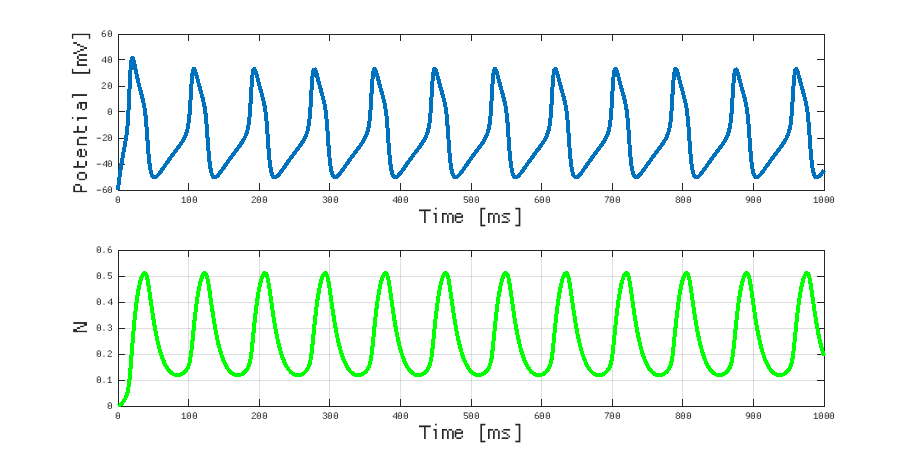
\includegraphics[width=\textwidth]{Figures/morris-lecar}
		\caption{Implementation of the fully deterministic Morris Lecar model. \textbf{TOP} Membrane potential. \textbf{Bottom} Fraction of open potassium channel.}
		\label{fig:morris-lecar}
	\end{figure}

	\subsection{Stochastic model}
	A finite number of potassium channels $N_{tot}$ is introduced and the number of open channels are treated as a discrete random process.
	Each potassium channel switches between the closed or open state independently of the other with voltage-dependent per capita transition rates $\alpha$ and $\beta$.
	The entire population conductance ranges from $0$ to $g_K^o = \frac{g_K}{N_{tot}}$.
	In this simulation $N_{tot} = 40$.
	The random variables will be the voltage and the number of open potassium channel.
	In the random time change representation the opening and closing of the potassium channels are driven by two independent unit rate Poisson processes $Y_{open}(t)$ and $Y_{close}(t)$.
	The evolutions  of $V$ and $N$ are linked.
	Whenever $N=n$, the evolution of $V$ obeys a deterministic differential equation:

	$$\frac{dV}{dt}\biggr\vert_{N=n} = f(V, n)$$

	$N$ evolves as a jump process: $N(t)$ is a piece-wise constant, with transitions occurring with intensities dependent on $V$.
	Whenever $V = v$:

	$$N\rightarrow N + 1\text{ net rate } \alpha(v)(N_{tot}-N)$$

	$$N\rightarrow N - 1\text{ net rate } \beta(v)N$$

	Now representing the state space for $N$ graphically:

	\begin{align*}
		0\xleftrightharpoons[\beta]{\alpha N_{tot}} 1 \xleftrightharpoons[2\beta]{\alpha(N_{tot}-1)}2\xleftrightharpoons[3\beta]{\alpha(N_{tot}-2)} \dots \xleftrightharpoons[k\beta]{\alpha(N_{tot}-k+1)}k&\\
		\scriptstyle{\alpha(N_{tot}-k)}\downharpoonleft\upharpoonright&\scriptstyle{(k+1)\beta}\\
		N_{tot}\xleftrightharpoons[N_{tot}\beta]{\alpha}(N_{tot}-1)\xleftrightharpoons[\beta(N_{tot}-1)]{2\alpha}\dots\xleftrightharpoons[(k+2)\beta]{\alpha(N_{tot}-k-1)}(k+1)&
	\end{align*}

The nodes represent possible states for process $N$ an the transition intensities located above and below the arrows.
Adopting the random time change representation the stochastic Morris-Lecar system is written as:

\begin{align*}
	\frac{dV}{dt} =& f(V(t), N(t)) = \\
								=& \frac{1}{C}(I_{app}-g_{Ca}m_\infty(V(t))(V(t)-V_{Ca})-g_L(V-V_L) +\\
								 &\qquad - g_K^oN(t)(V(t)-V_K))
\end{align*}

\begin{align*}
	N(t) = N(0) -&Y_{close}\biggl(\int_0^t\beta(V(s))N(s)ds\biggr) + \\
							 &Y_{open}\biggl(\int_0^t\alpha(V(s))(N_{tot}-N(s))ds\biggr)
\end{align*}

		\subsubsection{Random time change representation}
		We simulated the stochastic Morris Lecar model considering only the Potassium channel through the random time change representation for $4000$ seconds.
		The relationship within voltage and the number of open channel can be seen in figure \ref{fig:ml-rtc}.

		\begin{figure}
			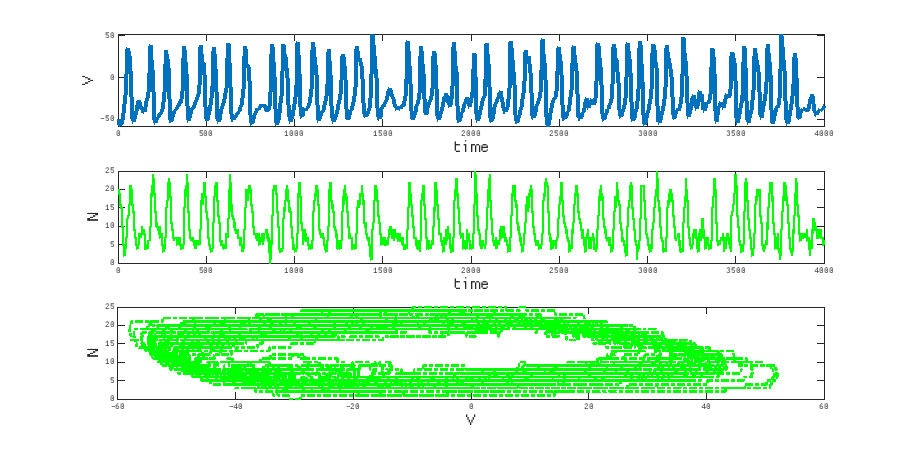
\includegraphics[width=\textwidth]{Figures/ml-rtc}
			\caption{The Morris Lecar stochastic model with only potassium channels. From top to bottom: \textbf{1} The membrane voltage. \textbf{2} The number of open potassium channel over time. \textbf{3} The number of open potassium channels over voltage.}
			\label{fig:ml-rtc}
		\end{figure}

		\subsubsection{Gillespie's representation}
		We simulated the stochastic Morris Lecar model considering only the Potassium channel through Gillespie's representation for $4000$ seconds.
		The relationship within voltage and the number of open channel can be seen in figure \ref{fig:ml-gill}.

		\begin{figure}
			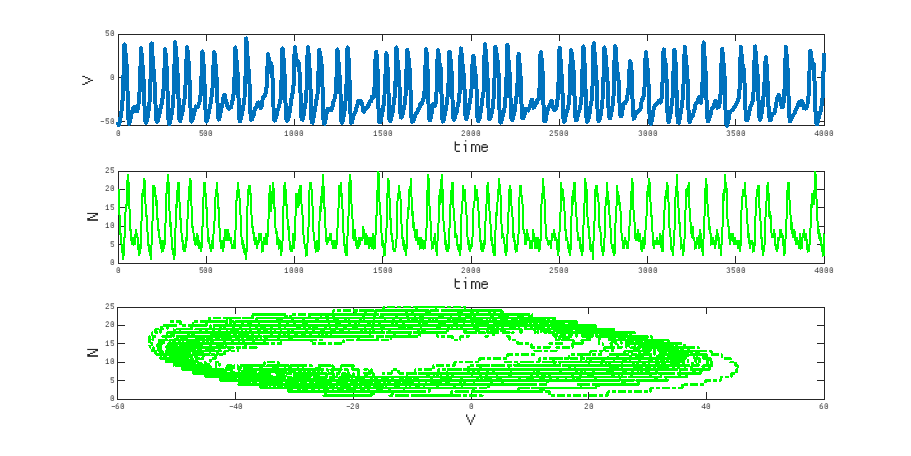
\includegraphics[width=\textwidth]{Figures/ml-gill}
			\caption{The Morris Lecar stochastic model with only potassium channels. From top to bottom: \textbf{1} The membrane voltage. \textbf{2} The number of open potassium channel over time. \textbf{3} The number of open potassium channels over voltage.}
			\label{fig:ml-gill}
		\end{figure}


\section{Models with more than one channel type}
Now the original Morris-Lecar model is considered, where there is a three-dimensional phase space.
In the original treatment of voltage oscillations  in barnacle muscle fibres the calcium gating variable $m$ is included as a dynamical variable, sot the total system is describes with the following deterministic equations:

\begin{align*}
	\frac{dv}{dt} = F(v, n, m) =&\frac{1}{C}(I_{app}-g_L(v-v_L)+\\
															&-g_{Ca}m(v-v_Ca)-g_Kn(v-v_K))
\end{align*}

\begin{align*}
	\frac{dn}{dt} &= G(v, n, m) = \alpha_n(v)(1-n)-\beta_n(v)n=\\
								&=\frac{n_{\infty}(v)-n}{\tau_n(v)}
\end{align*}

\begin{align*}
	\frac{dm}{dt} &= H(v, n, m) = \alpha_m(v)(1-m)-\beta_m(v)m=\\
								&=\frac{m_\infty(v)-m}{\tau_m(v)}
\end{align*}

The number of calcium gates evolves according to this equation instead of being set to its asymptotic value $m_\infty = \frac{\alpha_m}{\alpha_m+\beta_m}$.
The planar form of the equation is obtained by observing that $m$ approaches equilibrium faster than $n$ and $v$, so using standard arguments from singular perturbation theory this system can be brought into the planar model by replacing $F$ and $G$ with: $f(v, n) = F(v, n, m_\infty(v))$ and $g(v, n) = G(v, n, m_\infty(v))$.
Now for the $3D$ model $\epsilon_m = \frac{v-v_a}{v_b}$ has to be introduced in addition to $\epsilon_n = \frac{v-v_c}{v_d}$.
It can be noted how $\epsilon_x$ represents where the voltage falls along the activation curve for channel type $x$, relative to its half-activation point ($v_a$ for calcium and $v_c$ for potassium )and its slope (reciprocals of $v_b$ for calcium and $v_d$ for potassium).
The per capita opening and closing rates for each channel type are then:

$$\alpha_m(v) = \frac{\phi_m\cosh\frac{\epsilon_m}{2}}{1+e^{2\epsilon_m}}\quad\beta_m(v) = \frac{\phi_m\cosh\frac{\epsilon_m}{2}}{1+e^{-2\epsilon_m}}$$

$$\alpha_n(v) = \frac{\phi_n\cosh\frac{\epsilon_n}{2}}{1+e^{2\epsilon_n}}\quad\beta_n(v) = \frac{\phi_n\cosh\frac{\epsilon_n}{2}}{1+e^{-2\epsilon_n}}$$

With parameters:

\begin{multicols}{3}
	\begin{itemize}
		\item $v_a = -1.2$.
		\item $v_b = 18$.
		\item $v_c = 2$.
		\item $v_d = 30$.
		\item $\phi_m = 0.4$.
		\item $\phi_n = 0.04$
	\end{itemize}
\end{multicols}

The asymptotic open probabilities are given by $m_\infty$ and $n_\infty$ and the time constants $\tau_m$ and $\tau_n$, which satisfy the relations:

$$m_\infty(v) = \frac{\alpha_m(v)}{\alpha_m(v) + \beta_m(v)} = \frac{1+\tanh\epsilon_m}{2}$$

$$n_\infty(v) = \frac{\alpha_n(v)}{\alpha_n(v) + \beta_n(v)} = \frac{1+\tanh\epsilon_n}{2}$$

$$\tau_m(v) = \frac{1}{\phi\cosh\frac{\epsilon_m}{2}}$$

$$\tau_n(v) = \frac{1}{\phi\cosh\frac{\epsilon_n}{2}}$$

Assuming a population of $M_{tot}$ calcium and $N_{tot}$ potassium gates a stochastic hybrid system is obtained, with a continuous variable $V(t)$ and two discrete ones $M(t)$ and $N(t)$.
The voltage evolves according to the sum of the applied, leak, calcium and potassium currents

\begin{align*}
	\frac{dV}{dt} &=&  F(V(t), N(t), M(t)) = \\
								&=& \frac{1}{C}\biggl(I_{app} - g_L(V(t)-v_L)-g_{Ca}\frac{M(t)}{M_{tot}}(V(t)-v_{Ca}) +\\
								& &- g_K\frac{N(t)}{N_{tot}}(V(t)-v_K)\biggr)
\end{align*}

The number of open gates change only by unit increases and decreases remaining constant between such changes.
So the channel states evolve according to:

\begin{align*}
	M(t) =&M(0) - Y_{close}^M\biggl(\int_0^t\beta_m(V(s))M(s)ds\biggr)+\\
				&+Y_{open}^M\biggl(\int_0^t\alpha_m(V(s))(M_{tot}-M(s))ds\biggr)
\end{align*}

\begin{align*}
	N(t) =&N(0) - Y_{close}^N\biggl(\int_0^t\beta_n(V(s))N(s)ds\biggr)+\\
				&+Y_{open}^N\biggl(\int_0^t\alpha_n(V(s))(N_{tot}-N(s))ds\biggr)
\end{align*}

	\subsection{Deterministic representation}
	Firstly we analysed the trajectory of the fully deterministic model, which can be seen in figure \ref{fig:morris-lecar-4}.

	\begin{figure}
		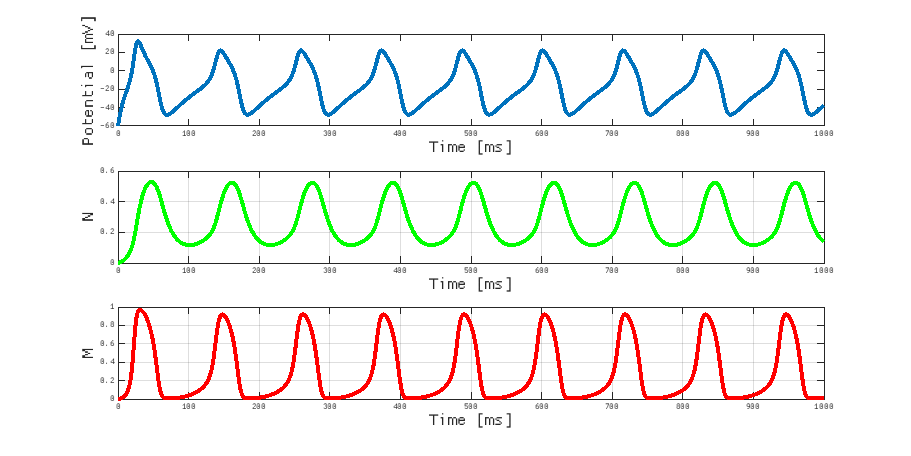
\includegraphics[width=\textwidth]{Figures/morris-lecar-4}
		\caption{Deterministic Morris Lecar model with evolving potassium and calcium dynamics. From top to bottom: \textbf{1} Membrane voltage. \textbf{2} Fraction of open potassium channels. \textbf{3} Fraction of open calcium channels.}
		\label{fig:morris-lecar-4}
	\end{figure}

	\subsection{Random time change representation}
	We simulated the stochastic Morris Lecar model  through the random time change representation for $4000$ seconds.
		The relationship within voltage and the number of open channel can be seen in figure \ref{fig:ml-rtc-4}.

		\begin{figure}
			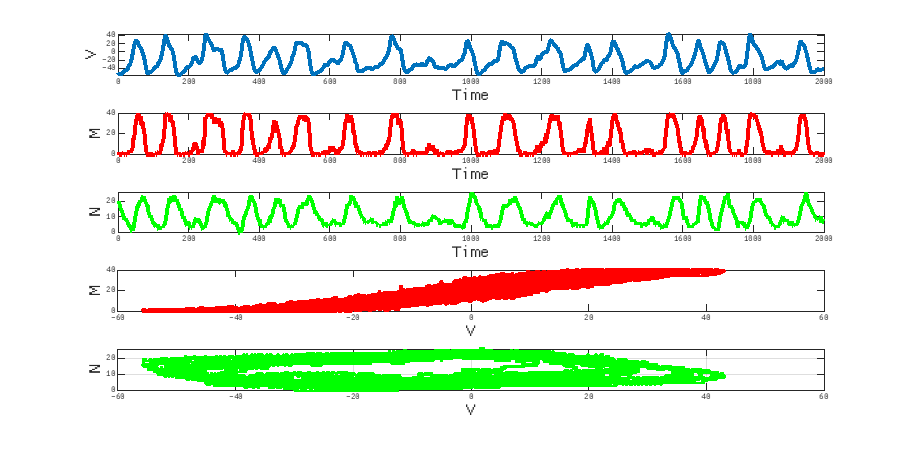
\includegraphics[width=\textwidth]{Figures/ml-rtc-4}
			\caption{The Morris Lecar stochastic model with only potassium channels. From top to bottom: \textbf{1} The membrane voltage. \textbf{2} The number of open calcium channel over time. \textbf{3} The number of open potassium channels over time. \textbf{4} The number of open calcium channel over voltage. \textbf{5} The number of open potassium channel over voltage}
			\label{fig:ml-rtc-4}
		\end{figure}

	\subsection{Gillespie's representation}
	We simulated the stochastic Morris Lecar model through Gillespie's representation for $4000$ seconds.
	The relationship within voltage and the number of open channel can be seen in figure \ref{fig:ml-gill-4}.

	\begin{figure}
		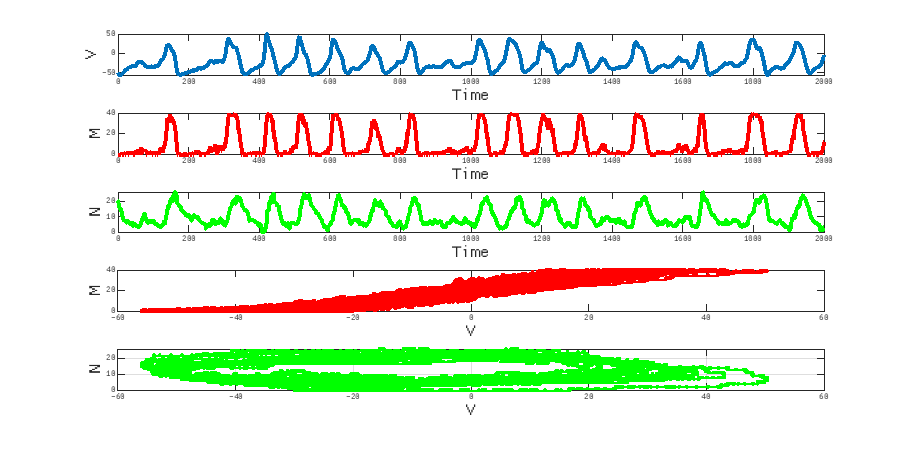
\includegraphics[width=\textwidth]{Figures/ml-gill-4}
		\caption{The Morris Lecar stochastic model with only potassium channels. From top to bottom: \textbf{1} The membrane voltage. \textbf{2} The number of open calcium channel over time. \textbf{3} The number of open potassium channels over time. \textbf{4} The number of open calcium channel over voltage. \textbf{5} The number of open potassium channel over voltage}
		\label{fig:ml-gill-4}
	\end{figure}


\section{Comparison of the exact algorithm with a piecewise constant propensity approximation}
The most common implementation for hybrid ion channel models is an approximate method in which the per capita reaction propensities are held fixed between channel events: in particular in algorithm \ref{algo:random-time-change-sim}, $\int_t^{t+\Delta k}\lambda_k(V(s), X(s))ds$ is replaced with $\Delta_k\lambda_k(V(t), X(t))$, leaving the remainder unchanged.
In this type of algorithms the sequence of channel states jumps is generated using the propensity immediately following the most recent jump rather than taking into account the time dependence of the reaction propensities due to the changing voltage.
This is analogous to the forward Euler method for the numerical solution of ordinary differential equations.
The solution of a stochastic differential equation with a given initial condition is a map from the sample space $\Omega$ to a space of trajectories.
In this context $\Omega$ is one independent unit rate Poisson process per reaction channel.
For the planar model a point in $\Omega$ amounts to fixing two Poisson process, $Y_{open}$ and $Y_{closed}$ to drive the transitions of the potassium channels.
For the full 3D model there are four processes:

\begin{multicols}{2}
	\begin{itemize}
		\item $Y_1 \equiv Y_{Ca, open}$.
		\item $Y_2 \equiv Y_{Ca, closed}$.
		\item $Y_3 \equiv Y_{K, open}$.
		\item $Y_4 \equiv Y_{K, closed}$.
	\end{itemize}
\end{multicols}

The exact algorithm provides a numerical solution of the map from $\{Y_k\}_{k=1}^4\in\Omega$ and initial conditions $(M_0, N_0, V_0)$ to the trajectory $(M(t), N(t), V(t))$.
The approximate piecewise algorithm gives a map from the same domain to a different trajectory $(\tilde{M}(t), \tilde{N}(t), \tilde{V}(t)$.
To make a pathways comparison the initial condition and the four Poisson processes are fixed and the resulting trajectories are compared.
Both algorithms produce a sequence of noise-dependent voltage spike with similar firing rates.
The two trajectories remain close together initially and the timing for the first spike is similar for both.
Over time discrepancies between the trajectories accumulate: the timing of the second and third spikes is different and before ten spikes the spike trains have become uncorrelated.
Even though the trajectories diverge the two processes could still generate sample paths with similar time-dependent or stationary distributions: the two algorithms could still be close in a weak sense.
Given $M_{tot}$ and $N_{tot}$ the density for the hybrid Markov process can be written as:

$$\rho_{m,n}(v,t) = \frac{1}{dv}Pr\{M(t) = m, N(t) = n, V\in[v, v+dv]\}$$

Obeying the master equation:

\begin{align*}
	\frac{\partial\rho_{m, n}(v, t)}{\partial t} =& - \frac{\partial(F(v, n, m)\rho_{m, n}(v, t))}{\partial v} +\\
																								&-(\alpha_m(v)(M_{tot}-m)+\beta_m(v)m+\\
																								&+\alpha_n(v)\cdot(N_{tot}-m)+\beta_n(v)n)\rho_{m, n}(v, t)+\\
																								&+(M_{tot}-m+1)\alpha_m(v)\rho_{m-1, n}(v, t)+\\
																								&+(m+1)\beta_m(v)\rho_{m+1, n}(v, t)+\\
																								&+(N_{tot}-n+1)\alpha_n(v)\rho_{m, n-1}(v,t)+\\
																								&+(n+1)\beta_n(v)\rho_{m, n+1}(v, t)
\end{align*}

With initial condition $\rho_{m,n}(v,0)\ge 0$ given by any integrable density such that $\in_{v\in\mathbb{R}}\sum\limits_{m,n}\rho_{m, n}(v, 0)dv \equiv 1$ and boundary conditions:$\rho\rightarrow 0$ as $|v|\rightarrow\infty$ and $\rho\equiv 0$ for either $m, n<0$ or $m> M_{tot}$ or $n>N_{tot}$.
The approximate algorithm does not generate a Markov process since the transition probabilities depend on the past rather than the present value of the voltage.
Because of this they do not satisfy the master equation, but it is plausible that they may have a unique stationary distributoin.

Looking the histograms in the $(v, n)$ plane with entries summed over $m$.
The algorithms were run with independent randomm number streams in the limit cycle regime ($I_{app} = 100$) fir $I_{max} \approx 200000$ time units, sampled every $10$.
Considering $N_{tot} = M_{tot} = k$, for $k<5$ the difference is obvious, while increasing $k$ the histograms become more and more similar.

Looking now at bar plots of the histograms with points projected on the voltage axis: entries summed over $m$ and $n$, the plots become increasingly similar the greater the $k$>

To quantify the similarity of the histogram the empirical $L_1$ difference between them has been computed.
For the full $(v, n, m)$ histograms and then for the collapsed voltage axis.
Let $\rho_{m,n}(v)$ and $\tilde{\rho}_{m, n}(v)$ denote the stationary distributions for the exact and approximate algorithms respectively.
To compare the two the $L_1$ distance between them is approximated:

$$d(\rho,\tilde{\rho}) = \int_{v_{\min}}^{v{\max}}\biggl(\sum\limits_{m=0}^{M_{tot}}\sum\limits_{n=0}^{N_{tot}}|\rho_{m, n}(v)-\tilde{\rho}_{m,n}(v)|\biggr)dv$$

Where $v_{min}$ and $v_{max}$ where chosen so that $F(v_{min}, n, m>0\land F(v_{max}, n, m)<0\forall m,n$.
Such value must exist since $F(v,n,m)$ is linear and monotonically decreasing for $v$ for any fixed pair of $(n,m)$.
For any exact simulation algorithm, once the voltage component falls between $v_{min}\le v \le v_{max}$ it remains in that interval for all time.

\section{Coupling, variance reduction and parametric sensitivities}
The random time change formalism can be used to develop new and faster computational methods with no loss in accuracy coupling two processes in order to reduce the variance and increase the speed of different natural estimatore.
Consider for example the computation of parametric sensitivities, which is a tool that allow to determine parameters to which a system output is most responsive.
Suppose that the intensity or propensity functions are dependent on some vectors of parameters $\theta$.
$\theta$, in our case, includes the membrane capacitance, the underlying number of channels of each type, the reversal potentials, the maximal conductance and the input current. We investigated how sensitively the average firing rate depends on $\theta$ for family of models $(V^\theta, X^\theta)$, parameterized by $\theta$ is considered, with stochastic equations:

$$\frac{d}{dt}V^\theta(t) = f(\theta, V^\theta(t), X^\theta(t))$$

$$X^\theta(t) = x_0^\theta + \sum\limits_kY_k\biggl(\int_0^t\lambda_k^\theta(V^\theta(s), X^\theta(s))ds\biggr)\zeta_k$$

Where $f$ is some function and all other notation is as before.
Some quantities depend on the entire sample path.
Let $g(\theta, V^\theta, X^\theta)$ be a path functional capturing the quantity of interest.
In order to evaluate the relative shift in expectation of $g$ due to a perturbation of the parameter vector, the estimation would be:


\begin{align*}
	\tilde{s} &=\epsilon^{-1}\mathbb{E}\bigl[g(\theta', V^{\theta'}, X^{\theta'})-g(\theta, V^\theta, X^\theta)\bigr]\approx\\
						&\approx\frac{1}{\epsilon N}\sum\limits_{i=1}^N\bigl[g(\theta', V_{[i]}^{\theta'}, X_{[i]}^{\theta'})-g(\theta, V_{[i]}^\theta, X_{[i]}^\theta)\bigr]
\end{align*}

Where:

\begin{itemize}
	\item $\epsilon= ||\theta-\theta'||$.
	\item $(V_{[i]}^\theta, X_{[i]}^{\theta})$ is the $i$th path generated with parameter $\theta$.
	\item $N$ is the number of sample paths computed for the estimation.
\end{itemize}

A finite difference and Monte Carlo sampling could be used to approximate the change in expectation.
If the paths $(V_{[i]}^{\theta'}, X_{[i]}^{\theta'})$ and $(V_{[i]}^\theta, X_{[i]}^{\theta})$ are generated independently, the variance of the estimator for $\tilde{s}$ is $O(N^{-1}\epsilon^{-2})$ and its standard deviation $O(N^{-\frac{1}{2}}\epsilon^{-1})$.
In order to reduce the confidence interval of the estimator to a target level of $\rho >0$:

$$N^{-\frac{1}{2}}\epsilon^{-1}\lesssim\rho\Rightarrow N \gtrsim\epsilon^{-2}\rho^{-2}$$

Which can be prohibitive.
Reducing the variance of the estimator can be achieved coupling the processes $(V_{[i]}^{\theta'}, X_{[i]}^{\theta'})$ and $(V_{[i]}^\theta, X_{[i]}^{\theta})$ so that they are correlated by constructing them on the same probability space.
Different approach to this problem are discussed in the next sections.

In our case, ${\theta}$, includes:

\begin{itemize}
	\item The membrane capacitance.
	\item The underlying number of channels of each type. 
	\item The reversal potentials.
	\item The maximal conductance and the input current.
\end{itemize}

So:

$$\theta = \begin{pmatrix} C & N_{K} & N_{Ca} & \vec{E} & \vec{g} & s\end{pmatrix}$$

We specifically investigated how the average firing rate ($g$) for 5 sample paths changes as a result of the variation of number of potassium and calcium channels. 
To do so we built a vector of $\theta$, $\Theta$, changing for each element the values of 

$$N_K = [1, 10, 20, 30, 40, 50, 60, 70, 80, 90, 100]$$ 

And 

$$N_{Ca} = [1, 10, 20, 30, 40, 50, 60, 70, 80, 90, 100]$$

To estimate the sensitivity of the models with regards to the change of the number of channels, we compared the two processes measuring the \tilde{s} function for each couple:

$$\tilde{s}(\theta_i, \theta_j) = (g(\theta_i, V, X), g(\theta_j, V, X): \theta_i, \theta_j\in \Theta$$

Then, to uncover the sensitivity with respect to each channel we summed over the variations of the other one and averaged over each step increase:

$$\langle\tilde{s}(\theta_i, \theta_j)\rangle = \frac{1}{11}\sum\limits_{i}^{10}\tilde{s}(\theta_{N_k = N_K[i]}\theta_{N_K= N_K[i+1]})$$

Analogously for $N_{Ca}$.
Then we computed the average sensitivity for each step increase as:

$$S = \langle\langle\tilde{s}(\theta_i,\theta_j\rangle\rangle$$

	\subsection{Spike detection}
	To compute the observable of interest $g$, we employed the spike detection algorithm presented in \cite{spike-detection}.
	This algorithm allows to compute the mid point of the spikes as to allow for a faster computation with respect to algorithms that find the peaks.
	The spikes are defined as the position where $V(t)$ is greater than a predefined threshold.

	\subsection{The common random number method}
	The common random number CRN method simulates processes according to Gillespie representation with the same Poisson process $Y$ and the same stream of random variables $\{\epsilon_i\}$. For this method:

	$$S_{K} = 0.079$$
	$$S_{Ca} = -0.013$$ 
	
 	\subsection{The common reaction path method}
	The common reaction path method CRP simulates both processes according to the same random time change representation with the same Poisson processes $Y_k$.
	One stream of uniform random variables for each reaction channel is created and used for the simulation of both processes. For this method: 

	
	$$S_{K} = 0.077$$
	$$S_{Ca} = -0.019$$ 

\section{Discussion}
The random time change representation can be useful to computational neuroscience as it allows for generalization of computational methods developed in the context of biochemistry, in which the propensities depend upon the state of the jump process only, so that variance reduction strategies become feasible.
The random time change approach avoids several approximations: for example in simulation algorithms based on a fixed time step chemical Langevin approach, it is necessary to assume that the increments in channel state are Gaussian distributed over an appropriate time interval.
However in exact simulation of small patches the exact algorithm visits states incompatible with the Gaussian increment approximation regardless of time step size.
Another algorithm found in literature is the piecewise constant propensity or approximate forward algorithm.
This ignore changes to membrane potential during the intervals between channel state changes.
As the sensitivity of ion channel opening and closing to voltage is fundamental these algorithm are not appropriate unless time between openings and closing is especially small.
This study restrict attention to the suprathreshold regime of the Morris-Lecar model, in which the applied current puts the system above the Hoph bifurcation marking onset of oscillations.
Spiking is not the result of noise-facilitated release.
Another study used eigenfunction expansion methods, path integrals and theory of large deviations to study spike initiation as noise facilitated escape problem in the excitable regime, as well as to incorporate synaptic currents into a stochastic network model using versions of the exact algorithm presented in this paper.
the usual separation-of-time scales picture breaks done: the firing rate obtained by 1D Kramers rate theory when the slow recovery variable (fraction of open potassium channels) is taken to be fixed does not match that obtained by direct simulation with the exact algorithm.
By considering a maximum likelihood approach to the 2D escape problem, spontaneous closure of potassium channels contributes significantly to noise induced escape than spontaneous opening of sodium channel.
The algorithm presented are applicable beyond the effects of channel noise on the regularity of action potential firing in a single compartment neuron model.
Exact simulation of hybrid stochastic models have been used to study spontaneous dendritic NMDA spikes, intracellular growth of the T7 bacteriophage and hybrid stochastic network models taking into account piecewise deterministic synaptic currents.
The latter example represents a significant extension of the neural master equation approach to stochastic population models.
The random time change representation extends naturally to scenarios in which each channel has a greater number of states, but it would be better to combine it with complexity reduction methods such as the stochastic shielding algorithm.
Analysis of algorithms combining stochastic shielding and the random time change framework are a promising direction for future research.




% \begin{figure}[hbt!]
% \centering
% \label{volcano}
% \end{figure}
